\documentclass{ip-lab}

\lablevel{n4}
\labnumber{Laboratorio 2}
\labtitle{Recorridos de matrices}

\makeheader

\begin{document}

\maketitle

\begin{sectionbox}{Preparación del ambiente de trabajo}
Cree un módulo \texttt{matrices.py} para las actividades de matrices.
\end{sectionbox}

\begin{sectionbox}{Actividad 1: Búsqueda en cuadrantes}

Escriba una función que reciba una matriz cuadrada de enteros positivos de tamaño mínimo $2\times 3$ y el nombre de un color. El color determina en qué cuadrante de la matriz se debe buscar. La función debe retornar el primer número en el cuadrante especificado que sea par, cuando se recorra por filas y luego por columnas. Si no existe tal número, debe retornar \texttt{None}.

La matriz se divide en seis cuadrantes nombrados por colores:

\textbf{Mitad superior de la matriz:}
\begin{itemize}
    \item \textbf{Rojo:} tercio izquierdo de columnas
    \item \textbf{Verde:} tercio central de columnas
    \item \textbf{Azul:} tercio derecho de columnas
\end{itemize}

\textbf{Mitad inferior de la matriz:}
\begin{itemize}
    \item \textbf{Amarillo:} tercio izquierdo de columnas
    \item \textbf{Naranja:} tercio central de columnas
    \item \textbf{Morado:} tercio derecho de columnas
\end{itemize}

\begin{center}
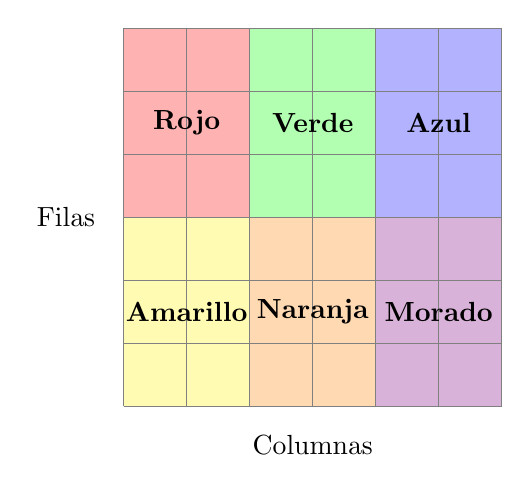
\begin{tikzpicture}[scale=0.8]
    % Draw grid
    \draw[step=1cm,gray,very thin] (0,0) grid (6,6);
    
    % Fill quadrants with colors
    \fill[red!30] (0,3) rectangle (2,6);
    \fill[green!30] (2,3) rectangle (4,6);
    \fill[blue!30] (4,3) rectangle (6,6);
    \fill[yellow!30] (0,0) rectangle (2,3);
    \fill[orange!30] (2,0) rectangle (4,3);
    \fill[violet!30] (4,0) rectangle (6,3);
    
    % Draw grid again on top
    \draw[step=1cm,gray] (0,0) grid (6,6);
    
    % Labels
    \node at (1,4.5) {\textbf{Rojo}};
    \node at (3,4.5) {\textbf{Verde}};
    \node at (5,4.5) {\textbf{Azul}};
    \node at (1,1.5) {\textbf{Amarillo}};
    \node at (3,1.5) {\textbf{Naranja}};
    \node at (5,1.5) {\textbf{Morado}};
    
    % Axis labels
    \node[below] at (3,-0.3) {Columnas};
    \node[left] at (-0.3,3) {Filas};
\end{tikzpicture}
\end{center}

\textbf{E.g.:} En una matriz 6x6, el cuadrante \verb|"verde"| abarca las filas 0-2 y columnas 2-3.

\end{sectionbox}

\pagebreak

\begin{sectionbox}{Actividad 2: Modificación de patrones}

Escriba una función que reciba una matriz cuadrada y la modifique pintando la letra "T".

\begin{itemize}
    \item La primera fila de la matriz debe contener únicamente el carácter \texttt{-}
    \item La columna del medio debe contener el carácter \texttt{|} desde la segunda fila hasta la última fila
    \item Todas las demás posiciones de la matriz deben contener el carácter espacio \texttt{' '}
\end{itemize}

Ejemplo para una matriz 5x5:

\begin{center}
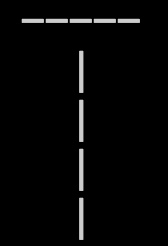
\includegraphics[width=0.4\textwidth]{matrix_t.png}
\end{center}

\end{sectionbox}

\pagebreak

\begin{sectionbox}{Actividad 3: Análisis de datos estructurados}

Escriba una función que reciba una tupla con información de ventas y el nombre de una ciudad, y retorne una tupla con el producto que tiene mayores ventas en esa ciudad y el valor de esas ventas.

La tupla de información contiene tres elementos:
\begin{itemize}
    \item Una matriz donde cada fila representa un producto y cada columna representa una ciudad
    \item Una lista con los nombres de los productos (en el mismo orden que las filas)
    \item Una lista con los nombres de las ciudades (en el mismo orden que las columnas)
\end{itemize}

Si la ciudad especificada no existe en los datos, la función debe retornar la tupla \texttt{(None, None)}.

\textbf{E.g.:} Si la matriz es \texttt{[[1500, 2000], [800, 1500]]}, los productos son \texttt{["Laptop", "Mouse"]}, las ciudades son \texttt{["Bogotá", "Medellín"]}, y se consulta por \texttt{"Medellín"}, la función debe retornar \texttt{("Laptop", 2000)} porque 2000 es mayor que 1500.

\end{sectionbox}

\pagebreak

\begin{sectionbox}{Actividad 4: Simulación de salón de clase}

Escriba una función que reciba una matriz cuadrada representando un salón de clase y retorne las coordenadas del primer estudiante introvertido que empezará a hablar en clase. Si ningún introvertido empezará a hablar, debe retornar \texttt{(None, None)}.

En la matriz, cada posición puede contener:
\begin{itemize}
    \item \texttt{0}: Puesto vacío
    \item \texttt{1}: Estudiante introvertido (callado)
    \item \texttt{2}: Estudiante extrovertido (hablando)
\end{itemize}

Un estudiante introvertido empezará a hablar si cumple estas dos condiciones simultáneamente:
\begin{enumerate}
    \item Tiene estudiantes extrovertidos en las dos posiciones diagonales inmediatamente detrás de él (diagonal inferior izquierda y diagonal inferior derecha). Si alguna de estas diagonales no existe porque el estudiante está en el borde del salón, esta condición no se cumple.
    \item La posición inmediatamente adelante no contiene un estudiante extrovertido. Si la posición adelante no existe porque el estudiante está en la primera fila, esta condición sí se cumple.
\end{enumerate}

El recorrido debe realizarse de adelante hacia atrás (de arriba hacia abajo) y de izquierda a derecha, como si estuviera mirando el salón desde el tablero.

E.g.: Si hay un introvertido en posición (1,1), tiene extrovertidos en (2,0) y (2,2), y la posición (0,1) no contiene un extrovertido, entonces ese introvertido empezará a hablar y sus coordenadas deben ser retornadas.

\end{sectionbox}


\begin{sectionbox}{Entrega}

Entregue el archivo a través de Bloque Neón en el laboratorio del Nivel 4 designado como ``N4-L2: Recorridos de matrices''.
\end{sectionbox}

\end{document}

